\subsection{Minimal filesystem}
\begin{frame}
  \frametitle{Basic applications}
  \fontsize{10}{10}\selectfont
  \begin{itemize}
  \item In order to work, a Linux system needs at least a few
    applications
  \item An \code{init} application, which is the first user space
    application started by the kernel after mounting the root
    filesystem (see \url{https://en.wikipedia.org/wiki/Init}):
    \begin{itemize}
    \item The kernel tries to run the command specified by the
          \code{init=} command line parameter if available.
    \item Otherwise, it tries to run \code{/sbin/init}, \code{/etc/init},
      \code{/bin/init} and \code{/bin/sh}.
    \item In the case of an initramfs, it will only look for
      \code{/init}. Another path can be supplied by the \code{rdinit=}
      kernel argument.
    \item If none of this works, the kernel panics and the boot
      process is stopped.
    \item The \code{init} application is responsible for starting all other
      user space applications and services, and for acting as a
      universal parent for processes whose parent terminate before they do.
    \end{itemize}
  \item A shell, to implement scripts, automate tasks, and allow a user
        to interact with the system
  \item Basic UNIX executables, for use in system scripts or in
        interactive shells: \code{mv}, \code{cp}, \code{mkdir}, \code{cat},
        \code{modprobe}, \code{mount}, \code{ip}, etc.
  \item These basic components have to be integrated into the root
    filesystem to make it usable
  \end{itemize}
\end{frame}

\begin{frame}
  \frametitle{Overall booting process}
  \begin{center}
    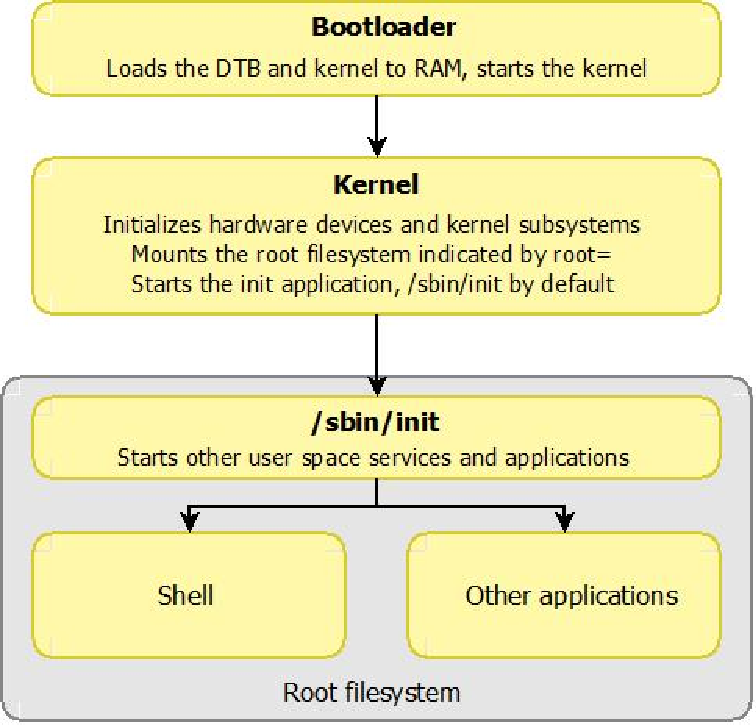
\includegraphics[height=0.8\textheight]{slides/sysdev-root-filesystem-minimal/overall-boot-sequence.pdf}
  \end{center}
\end{frame}
